\begin{figure*}[h!]
\scalebox{0.90}{
\begin{minipage}[t]{0.33\textwidth}
  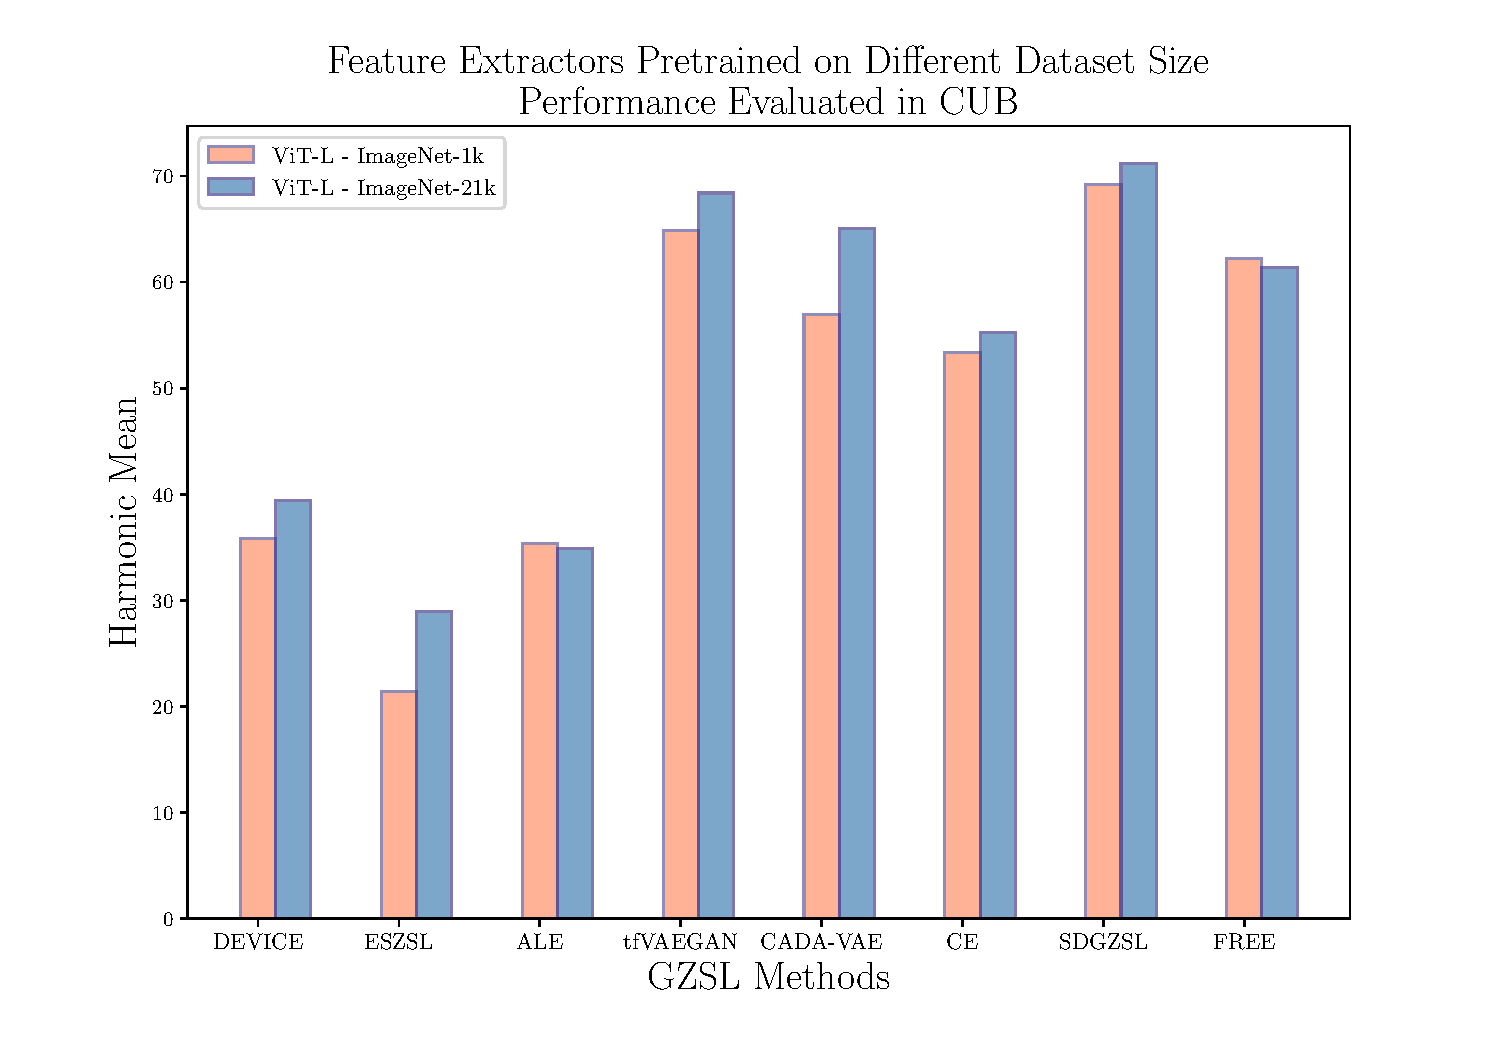
\includegraphics[align=t,width=\linewidth]{Images/cub_diff_data_size.pdf}
\end{minipage}%
\hfill % maximize the horizontal separation
\begin{minipage}[t]{0.33\textwidth}
  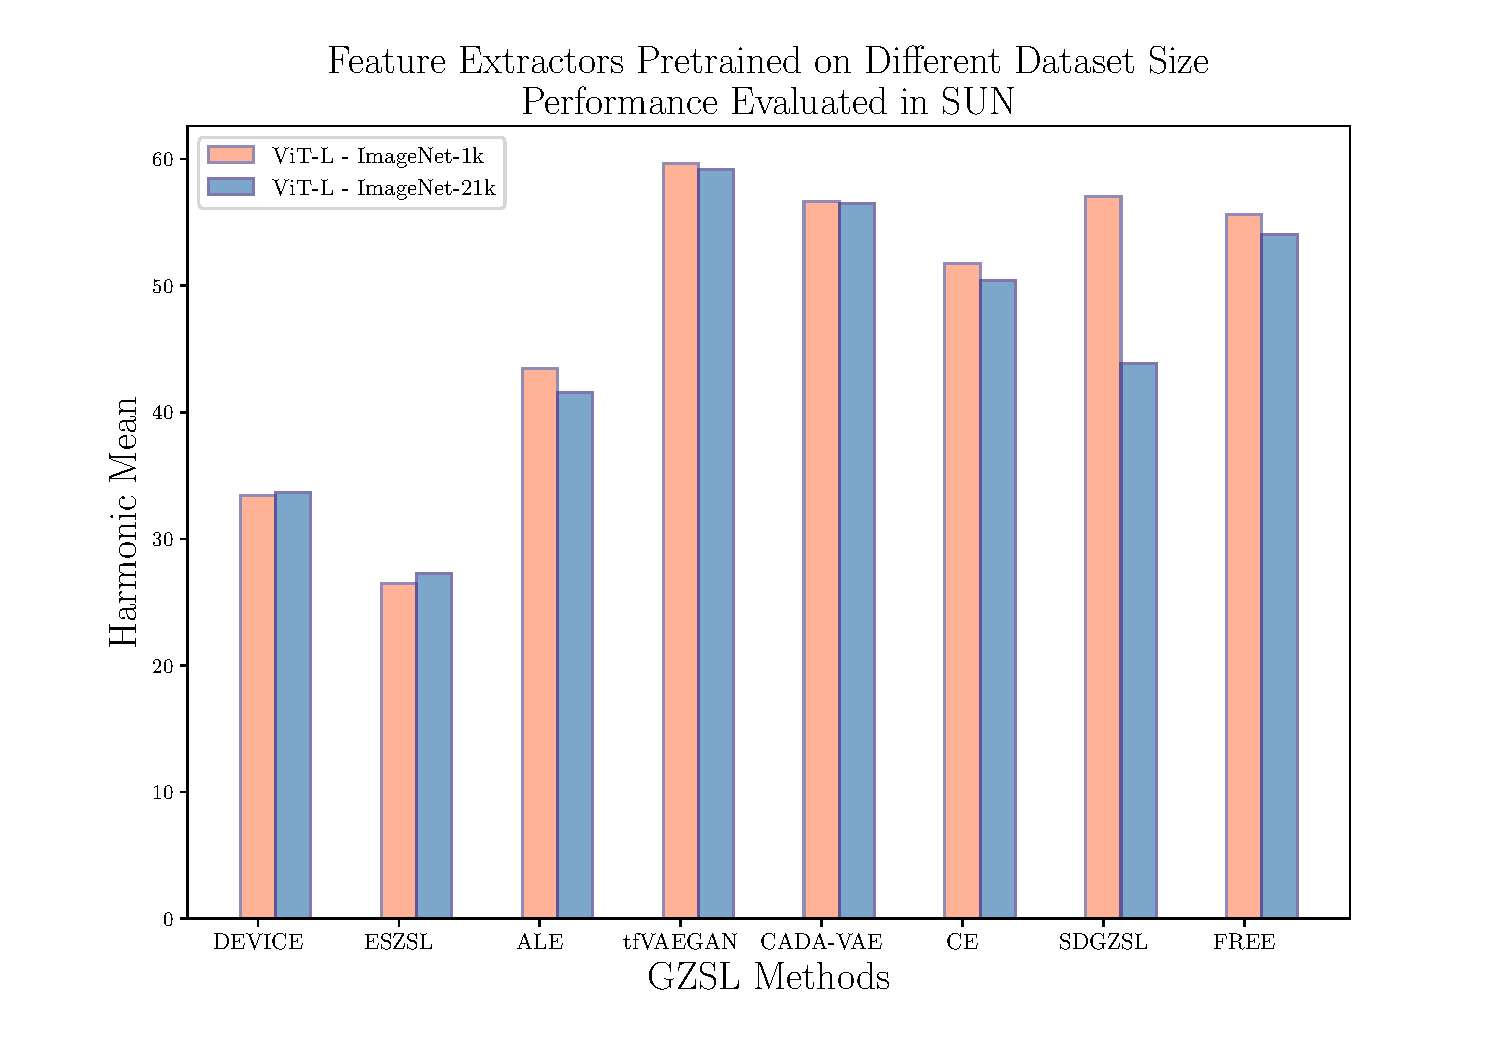
\includegraphics[align=t,width=\linewidth]{Images/sun_diff_data_size.pdf}
\end{minipage}%
\hfill
\begin{minipage}[t]{0.33\textwidth}
  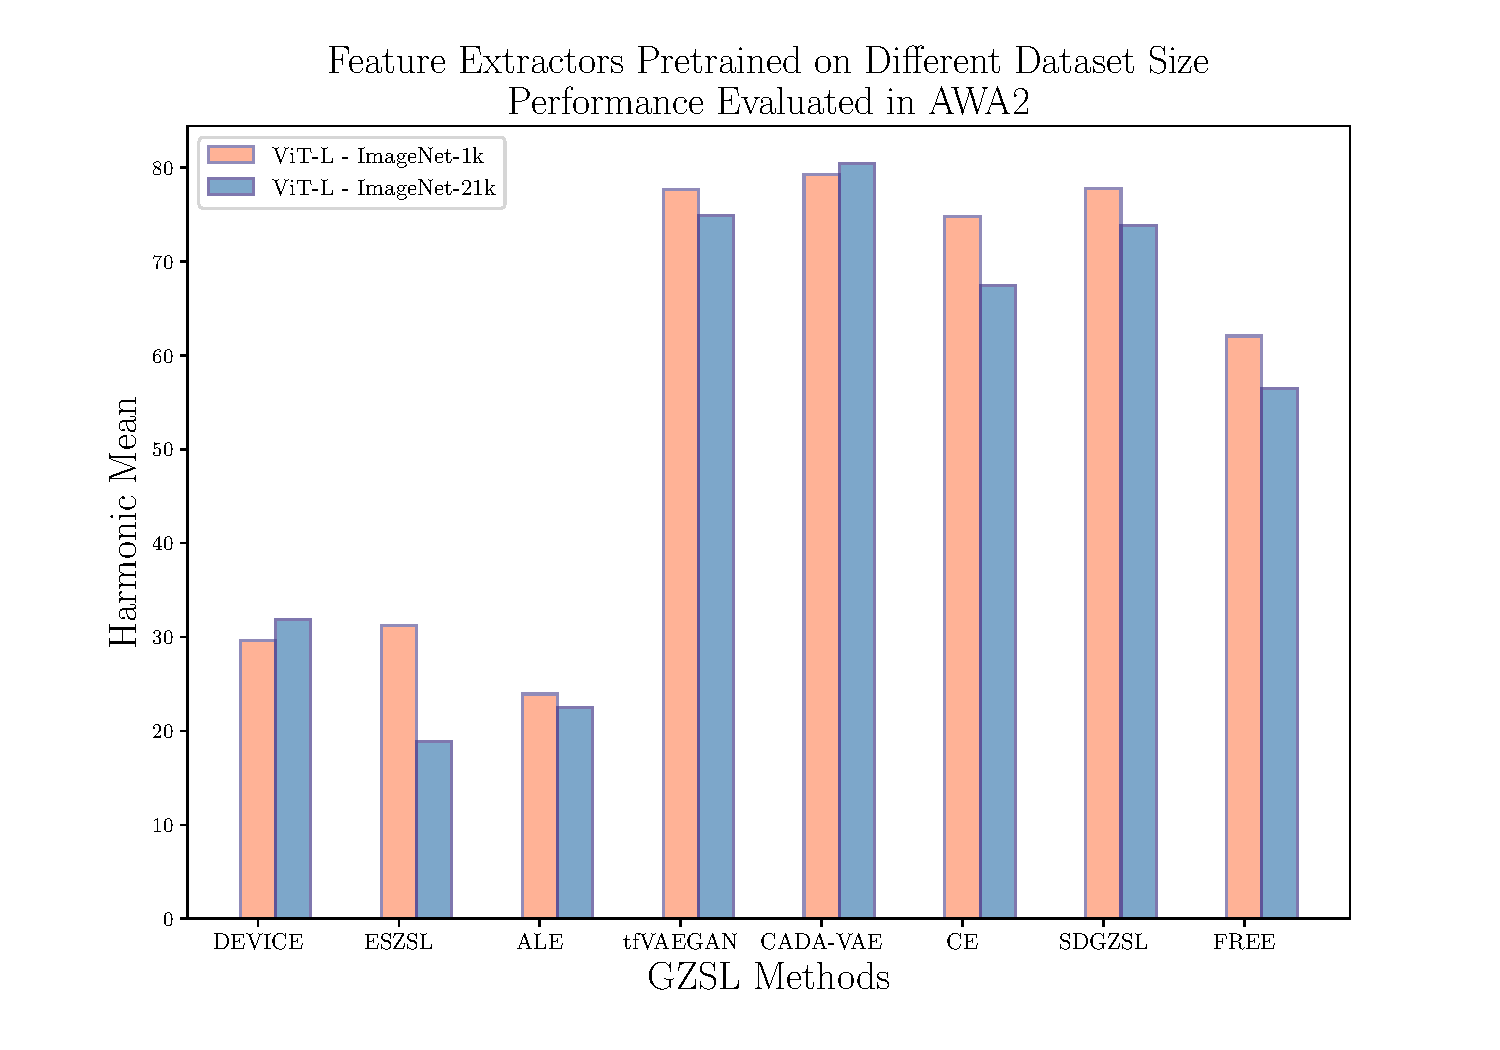
\includegraphics[align=t,width=\linewidth]{Images/awa2_diff_data_size.pdf}
\end{minipage}%
}
 \vspace{-0.05in}
 \caption{\textbf{Same Feature Extractor Pretrained with Different Datasets.} We show the Harmonic Mean performance of different GZSL methods when using a ViT$_{\text{Large}}$ model to extract the features of image samples from all datasets. [ViT-L - ImageNet-1k] and [ViT-L - ImageNet-21k] indicates the dataset the model was pretrained with. Best viewed in color.}
 \label{fig:model_backbone_data_size}
% \vspace{-0.05in}
\end{figure*}



\section{Pre-Trained Image Feature Extractors}

We begin our analysis by extracting the corresponding image features for all our samples using a diverse set of popular models pre-trained on Imagenet-1k and Imagenet-21k -- whose weights are publicly available. Prior work~\cite{AWA2} mention that using GoogLeNet features is not as effective as using Resnet101 features; thus, we want to further investigate: does feature extractor size matters for GZSL? This work aims to evaluate if pre-training on a bigger set impacts the outcomes, and if similarly robust features extracted from different model architectures -- other than Resnet101 -- makes a significant difference. 
For the backbones that were pre-trained using Imagenet-1k, we make sure that we use the same splits proposed in~\cite{AWA2} so that pre-trained features do not violate the zero-shot principle. 
We also want to measure the impact of using visual features extracted from networks that were pre-trained with data present in the test set of our settings. Thus, we investigate how the selected GZSL methods leverage the information extracted from larger backbones pre-trained with bigger and more diverse datasets (i.e., Imagenet-21k). 



